\chapter{Methodology And Proposed Framework}%
\label{chapter:methodology-and-proposed-framework}

\begin{introduction}
This chapter explains the research approach undertaken to tackle challenges of integrating \ac{NAUN3} devices into \ac{5G} networks. Outlines the specific methodologies employed for analysis of compatible authentication mechanisms as well as for managing device identity. Furthermore, it presents the designed framework for seamless, secure integration, detailing the motivation behind the architecture as well as essential building blocks.
\end{introduction}

\section{Overall Research Approach}

This research followed a constructivist methodology to develop a novel solution for integrating \ac{NAUN3} devices into \ac{5G} networks by repurposing existing \ac{5G} facilities and capabilities.

The initial phase involved a detailed study of the \ac{5G} architecture and relevant \ac{3GPP} standards. Although these standards include mechanisms for non-\ac{3GPP} access and for managing devices behind residential \acp{5G-RG}, they fall short of addressing the specific challenges posed by \ac{NAUN3} devices—particularly in terms of \ac{USIM} requirements and the inability to perform standard \ac{5G} authentication. The core issue identified was enabling \ac{5GC} acceptance, indirect authentication, and per-device handling without requiring changes to either the \ac{NAUN3} devices or the \ac{5GC} itself. Concepts such as \acp{CGID}~\cite{23.316-p27} and \ac{PDU} session separation were explored for inspiration, although detailed implementation strategies for such contexts are not specified in current standards.

To minimize required changes to both the \ac{5GC} and \ac{NAUN3} devices, the proposed solution centers on implementing all adaptation logic within the \ac{5G-RG}. This approach ensures transparency to both the core network and the end devices, while granting control to the network operator.

The central methodology involved designing a framework in which the \ac{5G-RG} acts as a mediator. This framework employs local authentication (specifically \ac{EAP-TLS}), with the \ac{5G-RG} serving as an authenticator that forwards requests to a mandatory, operator-controlled external \ac{EAP} server. This server authenticates devices lacking native \ac{5G} identities. Upon successful local authentication, the \ac{5G-RG} establishes a dedicated \ac{PDU} Session in the \ac{5GC} for each authenticated device. This session acts as a 'proxy identity', allowing the \ac{5GC} to manage the device's traffic without requiring direct knowledge of its non-\ac{5G} credentials. The \ac{5G-RG} also handles traffic forwarding between the device and its associated \ac{PDU} Session.

This framework, designed to meet integration requirements with minimal disruption, was subsequently detailed, prototyped in a testbed, and validated through functional and security testing, as elaborated in the following chapters. The approach was selected for its potential to deliver a practical, minimally invasive solution to the integration challenge.

\section{Requirements Analysis}

To address the challenge of integrating \ac{NAUN3} devices lacking native \ac{5G} credentials, while maintaining minimal disruption to existing systems, the following key requirements were defined to guide the framework design:

\begin{enumerate}
    \item {
        \textbf{Minimal Impact on Existing Infrastructure}
        \begin{enumerate}
            \item {
                \textbf{Core Network:} Standard \acl{5GC} functions (\acl{AMF}, \acl{SMF}, \acl{UPF}) must remain unaltered at the code level, with only configuration changes (e.g., \ac{IP} bindings, \ac{DNN} definitions) permitted.
            }
            \item {
                \textbf{End Devices:} \ac{NAUN3} devices must operate without hardware or software modifications, requiring only standard \ac{EAP} Supplicant functionality.
            }
            \item {
                \textbf{\acl{RAN}:} Standard \ac{5G} \ac{RAN} components (\acp{gNB}) must function without modification, maintaining standard interface operations with the core.
            }
        \end{enumerate}
    }
    \item {
        \textbf{\ac{5G-RG}-Centric Intelligence}
        \begin{itemize}
            \item {
                All adaptation logic must reside within the network's \ac{5G-RG}, which mediates between the \ac{NAUN3} device and the \ac{5GC}, in support of the minimal-impact goal.
            }
        \end{itemize}
    }
    \item {
        \textbf{Functional Requirements}
        \begin{itemize}
            \item {
                \textbf{Secure Device Onboarding:} Devices must be locally authenticated via \ac{EAP-TLS}, with the \ac{5G-RG} relaying requests to an operator-controlled external \ac{EAP} server.
            }
            \item {
                \textbf{Individual Device Representation:} Each authenticated device must be assigned a unique \ac{PDU} Session within the \ac{5GC}, serving as a proxy identity.
            }
            \item {
                \textbf{Traffic Separation:} Internal service traffic (e.g., \ac{RADIUS} communication) and end-device traffic must be clearly separated within the \ac{5G} transport network.
            }
            \item {
                \textbf{Lifecycle Management:} The \ac{5G-RG} must manage each device's session from initial authentication to disconnection, including re-authentication and \ac{PDU} Session teardown.
            }
            \item {
                \textbf{Traffic Mapping and Isolation:} The \ac{5G-RG} must ensure precise mapping and isolation of traffic between each device and its dedicated \ac{PDU} Session.
            }
        \end{itemize}
    }
    \item {
        \textbf{Operational Requirements}
        \begin{enumerate}
            \item {
                \textbf{Transparency:} The system must appear standard to both the \ac{5GC} (via \ac{PDU} procedures) and the \ac{NAUN3} device (via \ac{EAP} authentication).
            }
            \item {
                \textbf{Operator Manageability:} The complete solution, including \ac{5G-RG} logic and external \ac{EAP} infrastructure, must be operator-deployable and manageable.
            }
        \end{enumerate}
    }
\end{enumerate}

Together, these requirements establish the foundation for a solution that integrates unmodified \ac{NAUN3} devices into the \ac{5G} ecosystem with minimal disruption to existing network components and processes.


\section{Proposed Authentication Mechanism}

To securely onboard \ac{NAUN3} devices lacking native \ac{5G} credentials, this framework employs \ac{EAP-TLS}—a mutual certificate-based authentication method offering strong security and compatibility with standard operator-managed components like \ac{RADIUS} servers. \ac{EAP-TLS} is particularly suitable for \ac{IoT} devices, where password-based methods are often impractical or insecure. Figure~\ref{fig:EAP-TLS-topology} illustrates the architecture, which comprises three roles:

\begin{figure}
    \centering
    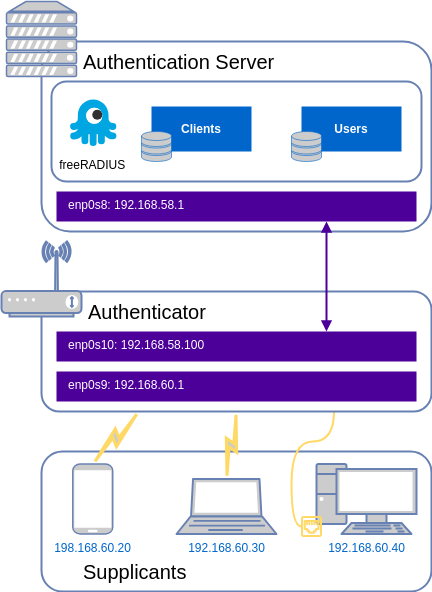
\includegraphics[width=0.5\linewidth]{figs/topology-EAP.png}
    \caption{\ac{EAP-TLS} Topology}
    \label{fig:EAP-TLS-topology}
\end{figure}

\begin{enumerate}
    \item {
        \textbf{Supplicant (\ac{NAUN3} Device):} Initiates the authentication using client-side \ac{EAP-TLS} and must be pre-provisioned with:
        \begin{itemize}
            \item A unique identity (e.g., username or \ac{MAC} address)
            \item A \ac{CA} certificate to validate the server
            \item A client certificate and private key (optionally password-protected)
        \end{itemize}
        Standard software such as \texttt{wpa\_Supplicant} is used to handle this role.
    }
    \item {
        \textbf{Authenticator (\ac{5G-RG}):} Acts as a relay, not terminating the \ac{EAP-TLS} session. Responsibilities include:
        \begin{itemize}
            \item Detecting device connection attempts
            \item Initiating the \ac{EAP} exchange (e.g., via \texttt{hostapd})
            \item Relaying \ac{EAP} messages over \ac{RADIUS} through the \texttt{backhaul} \ac{DNN}
            \item Maintaining device authentication states
            \item Triggering \ac{PDU} Session establishment upon successful authentication
        \end{itemize}
    }
    \item {
        \textbf{Authentication Server (e.g., FreeRADIUS):} Typically managed by the same \ac{ISP} operating the \ac{5GC}. Its functions are:
        \begin{itemize}
            \item Managing identities and issuing credentials
            \item Terminating and validating the \ac{EAP-TLS} session
            \item Authenticating clients via certificate verification
            \item Returning \ac{EAP}-Success or \ac{EAP}-Failure via \ac{RADIUS}
        \end{itemize}
    }
\end{enumerate}

\begin{figure}
    \centering
    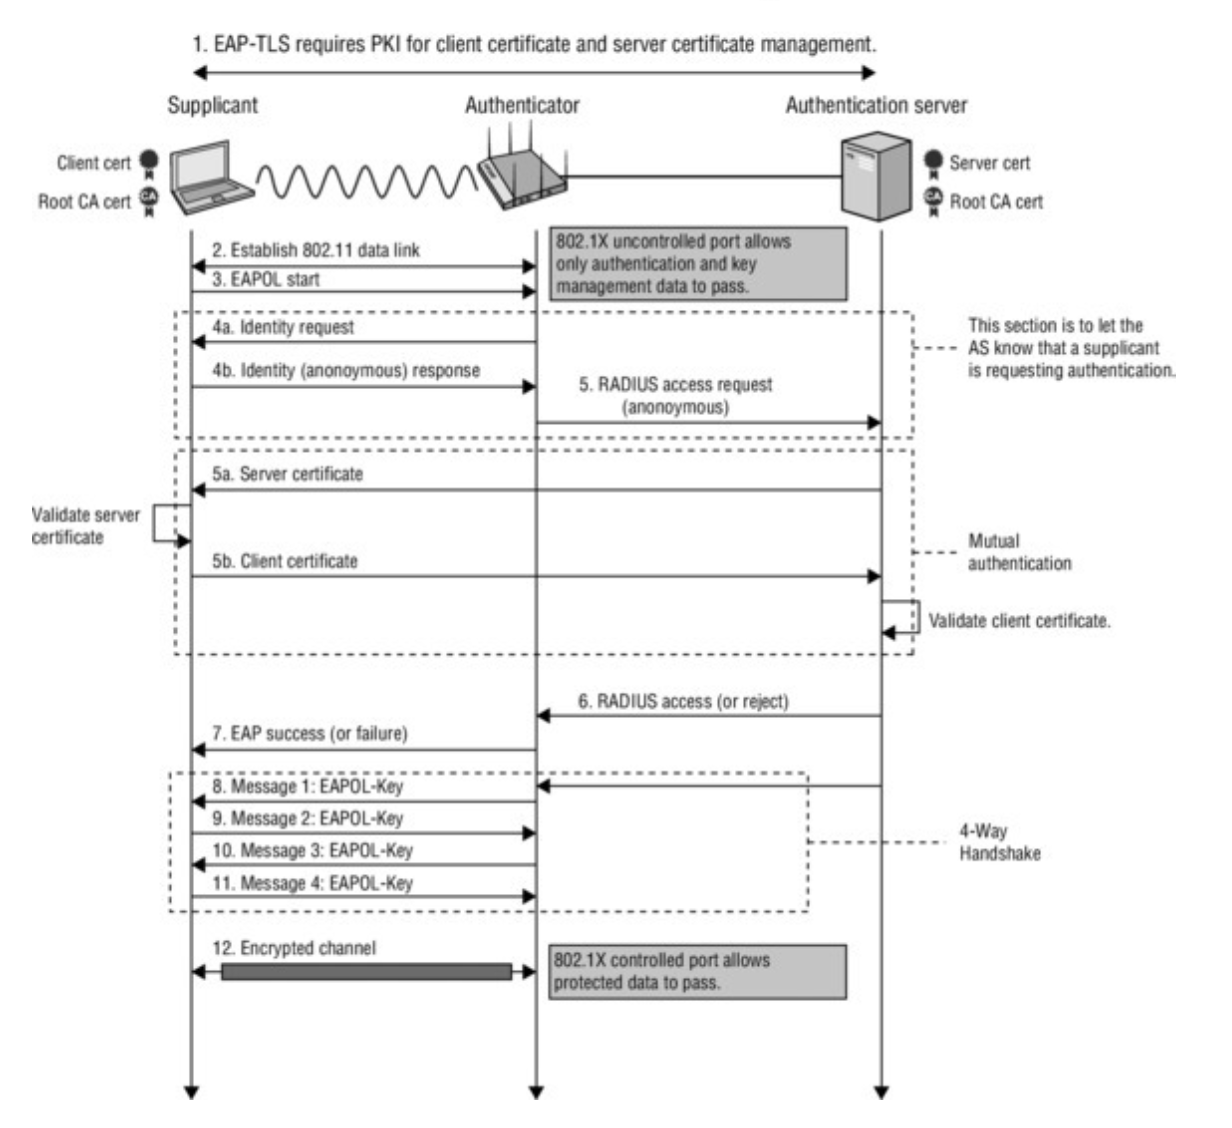
\includegraphics[width=0.75\linewidth]{figs/eap-tls-auth-flow.png}
    \caption{\ac{EAP-TLS} Authentication Flow}
    \label{fig:eap-tls-auth-flow}
\end{figure}

The \ac{EAP-TLS} authentication procedure, shown in Figure~\ref{fig:eap-tls-auth-flow}, follows these steps:

\begin{enumerate}
    \item Supplicant establishes a link-layer connection with the \ac{5G-RG} (e.g., via Wi-Fi or Ethernet).
    \item It sends an \ac{EAPOL}-Start to initiate authentication.
    \item The \ac{5G-RG} replies with an \ac{EAP}-Request/Identity.
    \item The Supplicant responds with an \ac{EAP}-Response/Identity (potentially anonymous).
    \item The \ac{5G-RG} relays this via a \ac{RADIUS} Access-Request to the Authentication Server.
    \item The server replies with its certificate inside an \ac{EAP}-Request (via Access-Challenge).
    \item The Supplicant validates the server certificate using its \ac{CA}.
    \item The client certificate is returned via \ac{EAP}-Response (also through Access-Challenge).
    \item Mutual authentication is completed when the server verifies the client certificate.
    \item The server sends \ac{RADIUS} Access-Accept with \ac{EAP}-Success (or Access-Reject with \ac{EAP}-Failure).
    \item The \ac{5G-RG} relays the final \ac{EAP} result to the Supplicant.
    \item If successful, a secure link-layer connection is established (e.g., \ac{WPA}2 4-Way Handshake).
\end{enumerate}

The \ac{5G-RG} interprets the final \ac{EAP} message as follows:

\begin{itemize}
    \item \textbf{\ac{EAP}-Success:} Triggers the \ac{5G-RG} to initiate a \ac{PDU} Session via the \texttt{clients} \ac{DNN}, binding the session to the authenticated device and handling traffic mapping.
    \item \textbf{\ac{EAP}-Failure:} Denies network access, terminating the process.
\end{itemize}

This mechanism assumes that devices are securely provisioned in advance with the required credentials. The provisioning process itself is considered out of scope for this implementation.

\section{Proposed Identity Management Solution}

Following the successful local authentication of a Wi-Fi-only/\ac{NAUN3} device, the next critical challenge is to enable its recognition and management within the \ac{5GC}.. This section details the proposed identity management solution, which innovatively utilizes the existing \ac{5G} \ac{PDU} session framework to create a dynamic, per-device proxy identity. This approach allows the \ac{5G-RG} to mediate connectivity and map individual devices to distinct network sessions, thereby integrating them transparently into the \ac{5G} ecosystem.

\subsection{The Identity Management Challenge}

The deployment of Wi-Fi-only, or \ac{NAUN3}, devices in the \ac{5G} network poses a fundamental identity management problem. Standard \ac{5G} identification depends on the \ac{SUPI}, usually derived from credentials stored securely in a \ac{USIM} (such as an \ac{IMSI} or \ac{NAI}). The \ac{SUPI} over the air is encrypted as a \ac{SUCI}. Devices without a \ac{USIM} cannot create a \ac{SUPI} or \ac{SUCI}, and hence cannot be recognized, verified, or managed via standard \ac{5GC} processes.

\subsection{Core Concept: \acs{PDU} Sessions as Proxy Identities}

To remedy this, the solution takes advantage of the capabilities of the \ac{5G-RG} and the versatility of \ac{5G} session management. From the viewpoint of the \ac{5GC}, a \ac{5G-RG} will act like a regular \ac{UE}, including its own \ac{USIM}, credentials, and support for several simultaneous \ac{PDU} Sessions. This allows segregation of traffic for different services or endpoints.

Taking a cue from the idea of \acp{CGID}, in which \ac{PDU} Sessions might represent a set of devices behind a gateway (collectively by \acp{SSID} or by Ethernet ports), the solution suggests a finer-grained approach: allocating each successfully authenticated \ac{NAUN3} device its very own dedicated \ac{PDU} Session, and not aggregating them.

In the proposed model, every \ac{PDU} Session, created and owned by the \ac{5G-RG}, will be a proxy identifier of a particular device. This enables not just integration into the \ac{5GC}, but also the ability to define session-specific controls and policies, and thus personalized management.

\subsection{Establishing the Proxy Identity}

After a device has been successfully authenticated through \ac{EAP-TLS}, as described in the earlier section, the \ac{5G-RG} then initiates a \ac{PDU} Session establishment procedure. This is done through its own credentials and \ac{SUPI}, to the \ac{SMF}, through the \ac{AMF}, and specifying the special-purpose \texttt{clients} \ac{DNN}.

Upon the assignment of resources — like an \ac{IP} address — by the \ac{5GC} to the session, the session is bound by the \ac{5G-RG} to the authenticated \ac{NAUN3} device. From there on, the session becomes the device’s operational identity in the \ac{5G} system.

\subsection{Gateway’s Role in Identity Mapping}

The \ac{5G-RG} maintains an internal mapping table that links each \ac{NAUN3} device’s local identifier (e.g., \ac{MAC} address) to its associated \ac{PDU} Session ID. This mapping enables accurate routing of data between the local network and the corresponding session within the \ac{5GC}.

\subsection{\ac{5GC} Perspective and Management}

From the point of view of the \ac{5GC}, the procedure is all standard. It communicates to just one registered \ac{UE}, the \ac{5G-RG}, to establish and release numerous \ac{PDU} Sessions related to the \texttt{clients} \ac{DNN}. Each session is managed by the \ac{SMF}, and it follows traditional techniques for resource assignment, policy control, and life cycle management.

Specifically, the \ac{5GC} has no knowledge of the device identities or the authentication information of the end devices behind the \ac{5G-RG}, it merely controls the session at the request of the gateway.

\subsection{Lifecycle of the Identity Mapping}

The \ac{5G-RG} takes charge of the entire life-cycle of the proxy identity:

\begin{itemize}
    \item \textbf{Creation:} Upon successful \ac{EAP-TLS} authentication of an \ac{NAUN3} device, the gateway creates a mapping entry and asks the \ac{5GC} to create a dedicated.
    
    \item \textbf{Maintenance:} The \ac{5G-RG} routes the device’s traffic through the corresponding \ac{PDU} Session and monitors the device’s local status (e.g., association state or heartbeat checks).

    \item {
        \textbf{Termination:} If the device disconnects or becomes inactive:
        \begin{enumerate}
            \item The gateway deauthenticates the device locally (e.g., via \texttt{hostapd}).
            \item It releases the associated \ac{PDU} Session via a standard release procedure to the \ac{5GC}.
            \item The internal mapping entry is removed.
        \end{enumerate}
    }
\end{itemize}

\subsection{Advantages of the Proposed Approach}

This session-based proxy identification scheme offers a number of beneficial features:

\begin{itemize}
    \item \textbf{Transparency:} The solution is transparent to both the \ac{NAUN3} device (which experiences usual local verification) and the \ac{5GC} (which maintains regular \ac{PDU} sessions).
    \item \textbf{Reuses Existing Infrastructure:} It constructs on top of existing \ac{5G} session management without the need to make any modifications to the core identity frameworks.

    \item \textbf{Localized Complexity:} Complexity of all sorts is centralized in the \ac{5G-RG}, reducing the need to integrate with.
    
    \item \textbf{Fine-Grained Control:} End-device \ac{PDU} Sessions support per-device policy enforcement (i.e., traffic shaping or \ac{QoS}) at the \ac{5GC}, providing fine-grained control.
\end{itemize}

\section{Framework Architecture and Integration}

\subsection{Overall Architecture Overview}

\begin{figure}
    \centering
    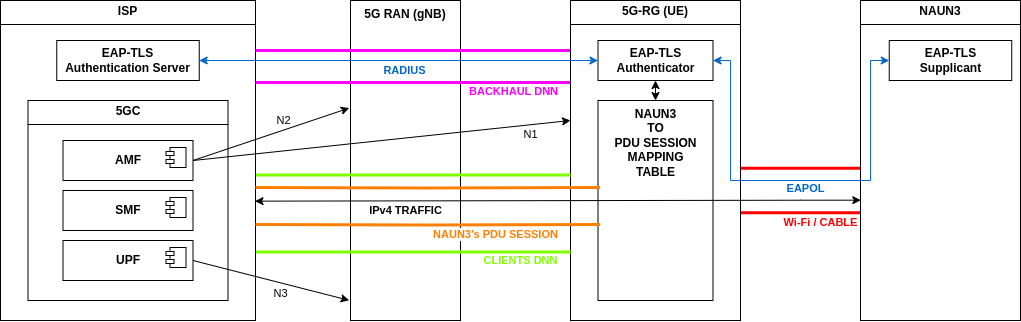
\includegraphics[width=1\linewidth]{figs/overall-topology.png}
    \caption{Overall Architecture}
    \label{fig:Overall Architecture}
\end{figure}

This top-level architecture Figure \ref{fig:Overall Architecture} shows the integration framework. The \ac{NAUN3} device connects locally (through Wi-Fi or cable) to the \ac{5G-RG}, the latter serving as a regular \ac{UE} to the \ac{gNB} and to the \ac{5GC} and serving as an \ac{EAP} Authenticator forwarding requests to the external \ac{EAP-TLS} Authentication Server within the domain of the \ac{ISP}. The connection between the \ac{5G-RG} and the \ac{EAP} server is done through the use of \ac{RADIUS}, over a dedicated \ac{PDU} session belonging to the \texttt{backhaul} \ac{DNN}. Most importantly, when the local authentication of the \ac{5G-RG} was successful, the latter creates a different \ac{PDU} session for the \ac{NAUN3} device.

\subsection{Interface and Protocol Integration}

A key aspect of this framework's design is its reliance on standard, well-defined interfaces and protocols, minimizing the need for proprietary extensions. The integration is achieved by orchestrating these standard elements in a specific manner, primarily through the logic implemented within the \ac{5G-RG}.

The main interfaces and protocols involved are:
\begin{itemize}
    \item {
        \textbf{Local Network Interface (between \ac{NAUN3} Device and the \ac{5G-RG}):}
        \begin{itemize}
            \item \textbf{Link Layer:} Standard Ethernet (\ac{IEEE} 802.3) or Wi-Fi (\ac{IEEE} 802.11).
            \item \textbf{Authentication:} Extensible Authentication Protocol over \ac{LAN} (\ac{EAPOL} - \ac{IEEE} 802.1X) is used to transport \ac{EAP} messages over the local link.
            \item \textbf{EAP Method:} \ac{EAP-TLS} is used for mutual authentication between the \ac{NAUN3} device (supplicant) and the \ac{EAP} infrastructure (via the \ac{5G-RG} relay).
        \end{itemize}
    }
    \item {
        \textbf{\ac{5G} Interfaces (between \ac{5G-RG} and the \ac{5GC}):}
        \begin{itemize}
            \item \textbf{N1 Interface:} Carries \ac{NAS} signaling between the \ac{5G-RG} and the \ac{AMF} for registration, authentication (of the \ac{RG} itself), and session management procedures.
            \item \textbf{N2 Interface:} Carries \ac{NGAP} signaling between the \ac{gNB}, which connects the \ac{5G-RG}, and the \ac{AMF}, primarily for \ac{UE} context management and \ac{PDU} session resource setup requests related to the \ac{5G-RG}.
            \item \textbf{N3 Interface:} Carries the user plane traffic encapsulated in \ac{GTP-U} tunnels between the \ac{gNB} and the \ac{UPF}. This includes traffic for both the \texttt{backhaul} \ac{PDU} session and all the individual \texttt{clients} \ac{PDU} sessions.
        \end{itemize}
    }
    \item {
        \textbf{Authentication Interface (between \ac{5G-RG} and the \ac{EAP} Authentication Server):}
        \begin{itemize}
            \item \textbf{Application Layer:} \ac{RADIUS} protocol is used to carry \ac{EAP} messages between the \ac{5G-RG} (acting as a \ac{RADIUS} client and \ac{EAP} authenticator) and the external authentication server).
            \item \textbf{Transport:} \ac{RADIUS} messages are transported over \ac{IP}, using \ac{UDP}. This \ac{IP} traffic is securely tunneled through the \ac{5G-RG}'s dedicated \texttt{backhaul} \ac{PDU} session via the N3 interface and \ac{UPF}.
        \end{itemize}
    }
\end{itemize}

The novelty lies not in modifying these protocols but in configuring the system components (\ac{5GC} \acp{NF}, \ac{5G-RG}, \ac{EAP} Server) and implementing the orchestration logic within the \ac{5G-RG} to manage the per-device proxy identity using standard \ac{5G} session management procedures.

\section{Scope and Assumptions}

This framework is able to bring \ac{NAUN3} devices into the \ac{5G} ecosystem by coordinating standard protocols and interfaces using smart logic centralized within the \ac{5G-RG}. Its main innovation is using individual \ac{PDU} Sessions, set up by the \ac{5G-RG}, as flexible proxy identities for each locally authenticated \ac{NAUN3} device. This method eliminates the need for devices to have native \ac{5G} credentials like \ac{SUPI} or \ac{USIM}.

Integration is handled dynamically across the device's connection lifecycle. After a device completes local \ac{EAP-TLS} authentication, the \ac{5G-RG} requests a dedicated \ac{PDU} Session (under the \texttt{clients} \ac{DNN}) from the \ac{5GC}. The \ac{5G-RG} keeps an internal mapping between the device's local identity and its assigned \ac{PDU} Session. If the device disconnects or loses connectivity, the \ac{5G-RG} promptly terminates the related \ac{PDU} Session to free up \ac{5G} resources, ensuring only active and authenticated devices consume network capacity.

Lastly, this setup enables the \ac{5GC} to manage each device individually—applying policies like \ac{QoS} and routing—through standard \ac{PDU} Session management, all without requiring changes to the \ac{NAUN3} devices or \ac{5G} core network functions. Integration relies entirely on configurations and the gateway's mediation, avoiding any need to alter fundamental \ac{5G} protocols or the capabilities of the devices themselves.